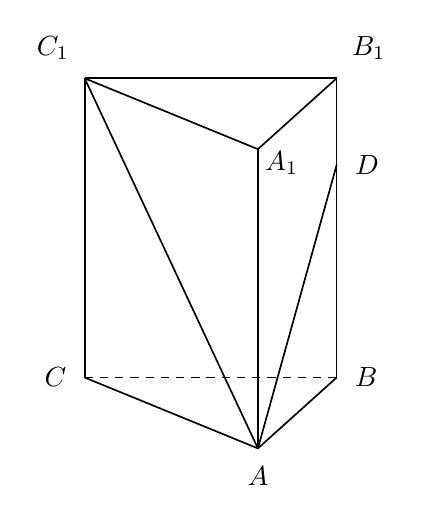
\begin{tikzpicture}[x=1cm,y=1cm,line width=0.6pt]
\coordinate (C1) at (0,5);
\coordinate (B1) at (3.2,5);
\coordinate (C) at (0,1.2);
\coordinate (B) at (3.2,1.2);
\coordinate (A) at (2.2,0.3);
\coordinate (A1) at (2.2000000000,4.1000000000);
\coordinate (D) at (3.2,3.9);
% top face
\draw[draw=black,solid] (C1) -- (B1);
\draw[draw=black,solid] (C1) -- (A1);
\draw[draw=black,solid] (B1) -- (A1);
% vertical side edges
\draw[draw=black,solid] (C1) -- (C);
\draw[draw=black,solid] (B1) -- (B);
\draw[draw=black,solid] (A) -- (A1);
% bottom face solid
\draw[draw=black,solid] (C) -- (A);
\draw[draw=black,solid] (B) -- (A);
% hidden bottom edge
\draw[draw=black,dashed,dash pattern=on 3pt off 2.5pt] (C) -- (B);
% interior diagonals
\draw[draw=black,solid] (C1) -- (A);
\draw[draw=black,solid] (A) -- (D);
% labels with clearance
\node[font=\normalsize,anchor=south east,xshift=-2pt,yshift=3pt] at (C1) {$C_{1}$};
\node[font=\normalsize,anchor=south west,xshift=2pt,yshift=3pt] at (B1) {$B_{1}$};
\node[font=\normalsize,anchor=east,xshift=-3pt,yshift=0pt] at (C) {$C$};
\node[font=\normalsize,anchor=west,xshift=3pt,yshift=0pt] at (B) {$B$};
\node[font=\normalsize,anchor=north,xshift=0pt,yshift=-3pt] at (A) {$A$};
\node[font=\normalsize,anchor=west,xshift=-1pt,yshift=-5pt] at (A1) {$A_{1}$};
\node[font=\normalsize,anchor=west,xshift=3pt,yshift=0pt] at (D) {$D$};
\end{tikzpicture}
